\section{Results}
% NOTE:
% You are expected to refer to all the floats (figures, tables, etc.)
% in the results section.
Write about your findings here.

% shows how to create a table and how to refer to it
Table~\ref{t:time} shows the average number of operations and elapsed
times (nanoseconds) for increasing input sizes.

\begin{table}[H]	% uses float package to control placement
	\centering	% centers the table
	\caption{
		The number of operations and the elapsed time (nanoseconds)
		as a function of the input size.
	}	% provides a concise description of the table contents

	\begin{tabular}{r r r}
		% table header
		size & operations & elapsed time \\
		% inserts horizontal line
		\hline
		% separates column entries with the ampersand &
		16 & 15 & 1460 \\
		32 & 31 &  757 \\
		64 & 63 &  606 \\
		128& 127&  949 \\
		256& 255& 1908 \\
		512& 511&  949
	\end{tabular}

	% defines a label to refer to it
	\label{t:time}
\end{table}


A graph of the average number of operations and the runtime is given in
figure~\ref{fig:best}.

\begin{figure}[H]
	% centers the figure
	\centering
	% my LaTeX installation expects Encapsulated PostScript EPS graphs
	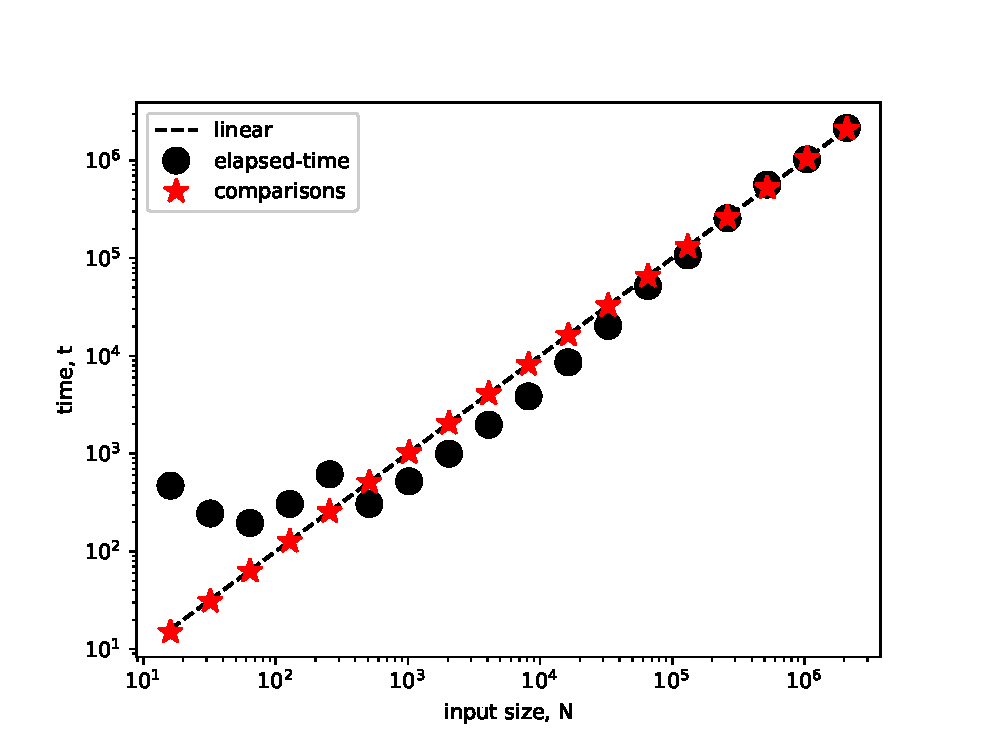
\includegraphics[keepaspectratio, width = 0.75\textwidth]{best.eps}
	\caption{
		The average number of operations and runtime as a
		function of the input size $N$.
	}
	% defines a label to refer to it
	\label{fig:best}
\end{figure}
